\documentclass[]{article}

\usepackage[margin=1.0in]{geometry}

% Line numbers
\usepackage{lineno}
\linenumbers

% Figures
\usepackage{graphicx}
\graphicspath{{figures/}}

% Trick Latex into placing all figures and tables at the end of the document
% regardless of their position in the source code.
\renewcommand{\textfraction}{1.0}
\renewcommand{\floatpagefraction}{0.9}

% Equations
\usepackage{amsmath}

% Bibliography
\usepackage{natbib}

% Better tables
\usepackage{booktabs}
\usepackage{multirow}
\newcommand{\ra}[1]{\renewcommand{\arraystretch}{#1}}


%--------------------------------------------------
% TITLE
%--------------------------------------------------
\title{SIO 217A: Cloud Droplet Growth}
\author{Team MecheE \\ Bengu Ozge Akyurek, David Larson, Guangchao Wang}
\date{\today}

\begin{document}

\maketitle


%--------------------------------------------------
% INTRO
%--------------------------------------------------
\section{Introduction}
Atmospheric thermodynamics focuses on water and its transformations. Advanced
topics are usually focused on phase transitions of water, homogeneous and
inhomogeneous nucleation, effect of dissolved substances on cloud condensation,
role of supersaturation on formation of ice crystals and cloud droplets.

Among those sub-topics, cloud nucleation is one area that
many researchers have worked on in the past several decades. Nucleation is
continually occurring in the atmosphere, both during gas-to-particle production
processes and in cloud formation which is a heterogeneous nucleation process
and involves nucleation centers or cloud nuclei.

People want to understand this process whereby a stable element of a new phase
first appears within the initial or parent phase for several reasons, one of
which is that the clouds have a very high albedo, and thus tend to reflect
incoming shortwave radiation back into space. Another reason that affects
atmospheric thermodynamics is that the nucleated clouds, as a new phase, could
produce precipitation, which is the primary route for water to move
geographically around the globe within the water cycle. To begin understanding
the larger effects of clouds, it is useful to analyze the growth of droplets in
warm clouds. This report discusses and evaluates one simplified model of
droplet growth rate.


%--------------------------------------------------
% MODEL
%--------------------------------------------------
\section{Cloud Droplet Growth}

\subsection{Model Description}
In order to model the cloud droplet growth as a function of time, we have used
Equation~\eqref{eq:5.26} from \cite{Curry}. This equation is based on
\cite{Mason}, which is based on \cite{Best}. The approximation assumes that a
droplet has the shape of a sphere that develops around a saturated nucleus
core. Furthermore, the environment conditions~(Temperature, pressure and
related parameters) are assumed to be constant, and the solute and curvature
effects are neglected, which will be explained in more detail. The initial
approximation is obtained by applying diffusion equations to the droplet, as
shown in Equation~\eqref{eq:Diffusion}.

\begin{equation}
    \label{eq:Diffusion}
    \dfrac{dm}{dt}=4 \pi r D_{v} \left( \rho_{v}(\infty) - \rho_{v}(r) \right)
\end{equation}

Adding the latent heat by condensation, shown in
Equation~\eqref{eq:LatentHeat}, gives the basis of the droplet growth rate
model.

\begin{equation}
    \label{eq:LatentHeat}
    \dfrac{dQ}{dt}=-L_{lv}\dfrac{dm}{dt}=-4 \pi r \kappa \left( T(\infty) - T(r) \right)
\end{equation}

These equations are combined to approximate the growth rate of a droplet by
diffusion as
\begin{align}
    \label{eq:5.26}
    r \frac{dr}{dt} = (S - 1) \left[ \frac{L_{lv}^2 \rho_l}{\kappa R_v T^2} + \frac{\rho_l R_v T}{e_s(T) D_v} \right] ^{-1} = \frac{S - 1}{K + D}
\end{align}
where $K$ and $D$ are the thermodynamic terms associated with heat conduction
and diffusion of water vapor, respectively. This differential equation is the
same as Equation 5.26 in \cite{Mason}. $S$ is the saturation ratio, $\rho_l$
the liquid density, $e_s$ the saturation pressure in the droplet and $T$ is the
environment temperature.

Assuming the atmospheric ambient conditions are constant (i.e. $T$, $S$, $K$,
and $D$ are constant), then Equation~\eqref{eq:5.26} can be integrated to get
\begin{align}
    \label{eq:5.27}
    r(t) = \left[ r_0^2 + \frac{2(S -1)}{K + D}(t - t_0)^2 \right] ^{1/2},
\end{align}
which can then be rearranged to find $t$

\begin{align}
    \label{eq:5.27T}
    t = (r^2 - r_0^2) \frac{K + D}{2(S - 1)}
\end{align}

Using the values from Table~\ref{tab:parameters}, the main results in
Table~\ref{tab:Table5.5} can be approximated. But to include the effects of
initial mass, curvature and the solute, we must modify our model.


\begin{table}[h]
    \centering
    \caption{Parameters for droplet growth rate.}
    \label{tab:parameters}

    \begin{tabular}{l l l l}
    \toprule
    Parameter & Value & Units & Notes\\
    \midrule
    $S - 1$   & 0.05            & \%                         & \\
    $p$       & 900             & $mb$                       & \\
    $T$       & 273             & $K$                        & \\
    $r_0$     & 0.75            & $\mu m$                    & \\
    $L_{lv}$  & 2.5x10$^{6}$    & $J \ kg^{-1}$              & pure water at $T=273 K$ \\
    $\rho_l$  & 1000            & $kg \ m^{-3}$              & pure water at $T=273 K$ \\
    $R_v$     & 461             & $J \ kg^{-1} K^{-1}$       & \\
    $\kappa$  & 2.4x10$^{-2}$   & $J \ m^{-1} s^{-1} K^{-1}$ & $T=273 K$ \\
    $D_v$     & 2.21x10$^{-5}$  & $m^2 s^{-1}$               & $T=273 K$, $p=1000 mb$ \\
              & 2.46x10$^{-5}$  & $m^2 s^{-1}$               & $T=273 K$, $p=900 mb$ \\
    $e_s (T)$ & 6.15            & $mb$                       & $T=273 K$\\
    \bottomrule
    \end{tabular}
\end{table}


\begin{table}[h]
    \centering
    \caption{Growth rate of droplets with nuclei of NaCl, ($S - 1$)=0.05\%,
        $p$=900mb, $T$=273K, and $r_0$=0.75$\mu$m recreated from Table 5.5 of \cite{Curry}.}
    \label{tab:Table5.5}

    \ra{1.2}
    \begin{tabular}{@{} c r r r @{}}
        \\
        \toprule
        m [g] & $10^{-14}$ & $10^{-13}$ & $10^{-12}$ \\
        \midrule
        r [$\mu$m] & \multicolumn{3}{c}{t [s]} \\
        \midrule
        1  & 2.4    & 0.15   & 0.013 \\
        2  & 130    & 7.0    & 0.61 \\
        4  & 1,000  & 320    & 62 \\
        10 & 2,700  & 1,800  & 870 \\
        20 & 8,500  & 7,400  & 5,900 \\
        30 & 17,500 & 16,000 & 14,500 \\
        50 & 44,500 & 43,500 & 41,500 \\
        \bottomrule
    \end{tabular}
\end{table}


One of the main properties of Equation~\eqref{eq:5.27T} is that it does not
depend on the nucleus mass, which directly contradicts with
Table~\ref{tab:Table5.5}. This led us to the first modification on the
approximation Equation~\eqref{eq:5.27T}. Rather than starting from
$r=r_{0}=0.75\ 10^{-6} \mu m$ and $t_{0}=0$ as given in the conditions of
Table~\ref{tab:Table5.5}, we have altered the definition of the starting radius
as the radius of the nucleus without any water. We haven't changed the value of
$r_{0}$, as this was given as one of the constants. But, we have defined
$t_{0}$ as the time the radius of the droplet develops to $r_{0}$, which is
definitely not $0$.

To calculate the initial radius, we have assumed that the nucleus is a perfect
sphere. Thus, the initial radius can calculated by
Equation~\eqref{eq:InitialRadius}.

\begin{equation} \label{eq:InitialRadius} \rho_{NaCl}\frac{4}{3}\pi
    r_{i}^{3}=m_{NaCl} \end{equation}

We have used $\rho_{NaCl}=2160 \frac{kg}{m^{3}}$. This adjustment introduced an
effect of the nucleus mass and decreased the overall error of the first given
approximation.

The secondary improvement was on $e_{s}$. The approximation assumed $e_{s}$ to
be a constant, but normally it is not. Especially for small $r$ values,
\cite{Best} states that $e_{s}$ deviates from its average value significantly.
Since our starting point involves small values of $r$, we have applied two
modifications on $e_{s}$. The first adjustment is the usage of Raoult's law to
incorporate the effect of surface tension, introducing an additional factor
depending on both $r$ and the mass of the nucleus. This factor is shown in
Equation~\eqref{eq:RaoultsLaw}. $i$ is a constant depending on the molecular
structure of the nucleus core and is taken as $i=2$. $e_{s\infty}$ is the
saturation pressure of the environment (at a virtual radius of $r=\infty$).

\begin{equation}
    \label{eq:RaoultsLaw}
    \dfrac{e_{s}}{e_{s\infty}}=\dfrac{n_{H2O}}{i n_{solt}+n_{H2O}}=\dfrac{\dfrac{\dfrac{4}{3}\pi r^{3} \rho_{H2O}}{M_{H2O}}}{i \dfrac{m_{solt}}{M_{solt}} + \dfrac{\dfrac{4}{3}\pi r^{3} \rho_{H2O}}{M_{H2O}}}
\end{equation}

The second modification is the introduction of the effect of curvature, which
is shown in Equation~\eqref{eq:Curvature}.

\begin{equation}
    \label{eq:Curvature}
    \dfrac{e_{s}}{e_{s\infty}}=\exp \left( \dfrac{2\sigma_{lv}}{\rho_{l}R_{v}Tr} \right)
\end{equation}

The combined effect of surface tension and the curvature are given in
Equation~\eqref{eq:EsDefinition}. Throughout our calculations and simulations,
we assume $T$ to be constant as its deviations from its initial value is
negligible. This modification in $e_{s}$ directly affects our $D$ value in
Equation~\eqref{eq:5.26}.

\begin{equation}
    \label{eq:EsDefinition}
    e_{s}(r,T)=e_{s\infty}\left(\dfrac{\dfrac{\dfrac{4}{3}\pi r^{3} \rho_{H2O}}{M_{H2O}}}{i \dfrac{m_{solt}}{M_{solt}} + \dfrac{\dfrac{4}{3}\pi r^{3} \rho_{H2O}}{M_{H2O}}}\right) \exp \left( \dfrac{2\sigma_{lv}}{\rho_{l}R_{v}Tr} \right)
\end{equation}

A final modification has been applied on the numerator $(S-1)$ of
Equation~\eqref{eq:5.26} as recommended by \cite{Mason}. The numerator is
redefined in Equation~\eqref{eq:Numerator} to add surface tension and curvature
effects, where $n$ represents the mole number of the material in the subscript.

\begin{equation}
    \label{eq:Numerator}
    (S-1) \rightarrow (S-1)+\dfrac{2\sigma_{lv}}{\rho_{l}R_{v}Tr}-\dfrac{i n_{solt}}{i n_{solt}+n_{H2O}}
\end{equation}

Although this equation increases the accuracy of the results, it depends itself
on $r$. This means that the simple quadratic solution in
Equation~\eqref{eq:5.27T} can not be used any more and we need a numerical
integration method to solve the differential equation in
Equation~\eqref{eq:5.26}. The explicit Euler method has been used for
integration. The iterative steps are defined in Equation~\eqref{eq:Iteration}.

\begin{equation}
    \label{eq:Iteration}
    r_{k+1}= \dfrac{S - 1+\dfrac{2\sigma_{lv}}{\rho_{l}R_{v}Tr}-\dfrac{n_{solt}}{i n_{solt}+n_{H2O}}}{K(T) + D(r_{k},T)}\dfrac{\Delta t}{r_{k}}
\end{equation}

The initial condition at $k=0$ is $r=r_{i}$ which was calculated as the radius
of the nucleus core itself.

Although this approximation is close to the values in Table~\ref{tab:Table5.5},
it has its drawbacks with respect to reality. The first limitation is that we
have assumed the temperature to be constant throughout the droplet and same as
the environment at all times. The second drawback is that we have assumed that
the environment properties like $\kappa, D_{v}, L_{lv}$ stay constant, which
introduces an extra error into our approximation.

Another drawback is due to the numeric integration error. We have computed the
symbolic integral via Wolfram and compared its result with the numeric
integration result, but the difference was small enough to be negligible. An
insignificant approximation is on the shape of both the nucleus core and the
droplet, as these will deviate from spheres in real cases.


\subsection{Model Parameters}
$K$ is the thermodynamic term related to the latent heat release due to
condensation and diffusion of heat away from the droplet. It depends on the
ambient temperature $T$, latent heat of vaporization $L_{lv}$ and the thermal
conductivity coefficient $\kappa$. $\rho_l$ denotes the water density.
$\kappa$ is the coefficient of thermal conductivity in air and increases with
increasing temperature to account for the faster heat conduction at higher
temperatures due to the higher kinetic energy of the air molecules.

$D$ is the vapor diffusion term related to the diffusion of water vapor onto
the growing droplet. It depends on the saturation vapor pressure $e_{s}$,
temperature $T$, and the coefficient of water vapor diffusion in air $D_v$.
$D_v$ increases with increasing temperature but decreases with increasing
pressure. An increase in pressure means a decrease in the mean free path of the
molecules so that collisions with other molecules and particles occur more
frequently. The increase of  $D_v$ with increasing temperature again accounts
for the faster diffusion at higher temperatures.

In addition, $S$ is saturation ratio. If $S$ is less than 1, the growth rate
$\frac{dr}{dt}$ is less than 0, which describes the evaporation of a cloud
drop. Conversely, $S$ greater than 1 describes the condensation of a cloud
drop.

In Equation~\eqref{eq:5.27}, $K$ depends on temperature and $D$
depends on temperature and pressure. The higher the temperature, the smaller is
the term $K$. $D$ has temperature dependent terms both in the numerator and in
the denominator. Here the temperature dependence in the denominator dominates
so that $K$ also decreases with increasing temperature. This means that the
denominator is smaller for higher temperatures, i.e.\ the droplets grow or
shrink faster at higher temperatures for a given saturation ratio $S$. This is
intuitive because at higher temperature, the absolute difference in water vapor
pressure between the droplet surface and its surroundings is higher for a given
saturation ratio, and therefore also the water vapor pressure gradient at the droplet
surface, which drives diffusional growth or evaporation of the droplet.

Diffusive transport in droplet growth process is smaller than advective
transport, but plays an important role in the process because water vapor is
diffused towards the cloud drop, and heat is diffused away from the cloud drop.
In sum, the droplet growth rate is a function of saturation ratio over the sum
of rate of transfer of water vapor to the droplet and rate of transfer of
latent heat of condensation away from the droplet.


%--------------------------------------------------
% RESULTS
%--------------------------------------------------
\section{Results of Modeling Study}
Figure~\ref{fig:r_t} shows a visual comparison between the droplet growth rate
modeled by Equation~\eqref{eq:5.27} with $r_0 = 0.75 \mu m$, $T=273 K$, $p=900
mb$, and $(S - 1) = 0.05\%$. A major assumption of Equation~\eqref{eq:5.27} is
that the curvature and solute effects are neglible once the droplet grows
beyond a few microns. The figure shows general agreement between the model and
values from Table 5.5 of \cite{Curry}.

\begin{figure}[h]
    \centering
    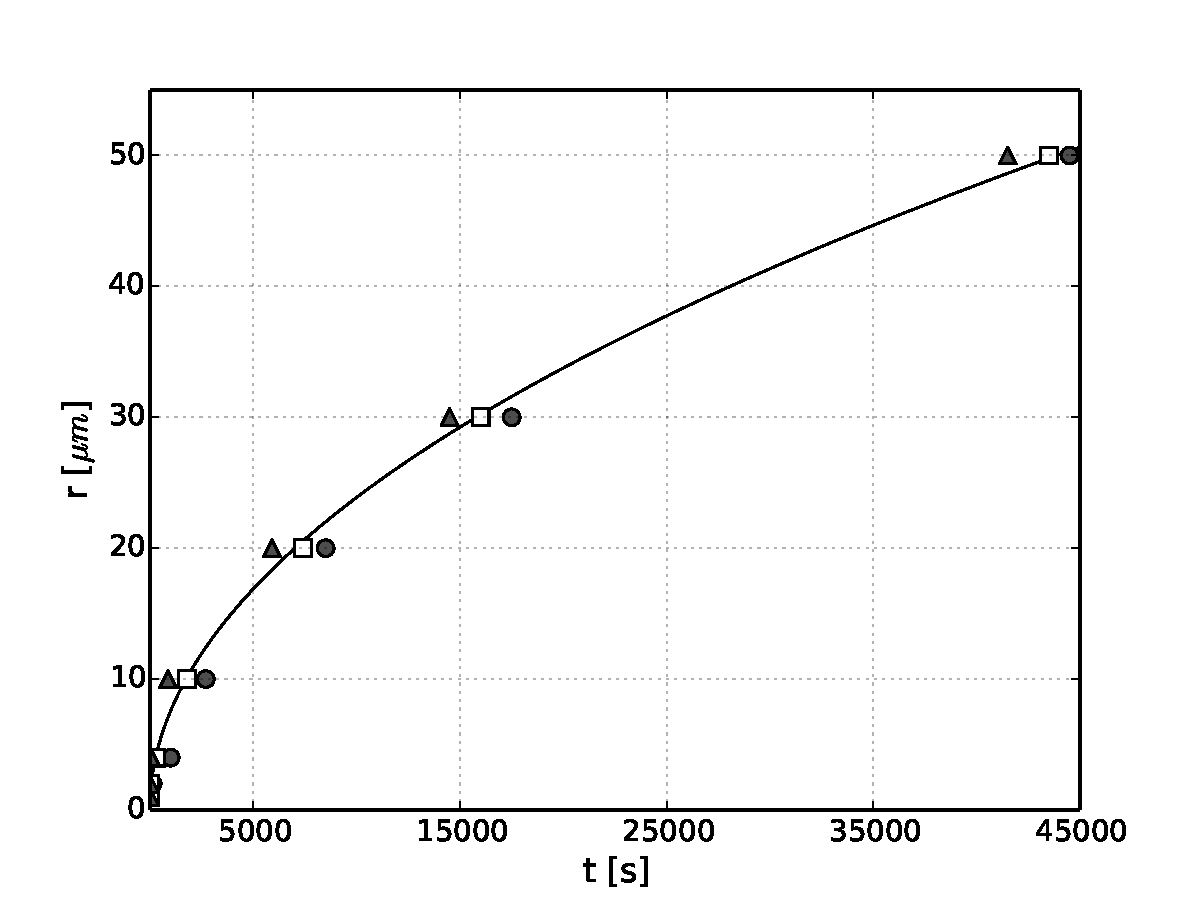
\includegraphics[width=\textwidth]{r_t.pdf}
    \caption{Droplet growth rate of the simplified model against the values from Table 5.5 of \cite{Curry}.}
    \label{fig:r_t}
\end{figure}


To study the sensitivity of the model, we varied $T$ and $(S - 1)$, separately,
while holding all other parameters constant. Figure~\ref{fig:temperature} and
~\ref{fig:supersaturation} show the results.  Increasing $T$ increases the
droplet growth rate, due to decreased values of $K$ and increased values of
$D$.  Likewise, increasing $(S - 1)$ increases the droplet growth rate due to
an increased amount of water vapor, which lowers the activation.

\begin{figure}
    \centering
    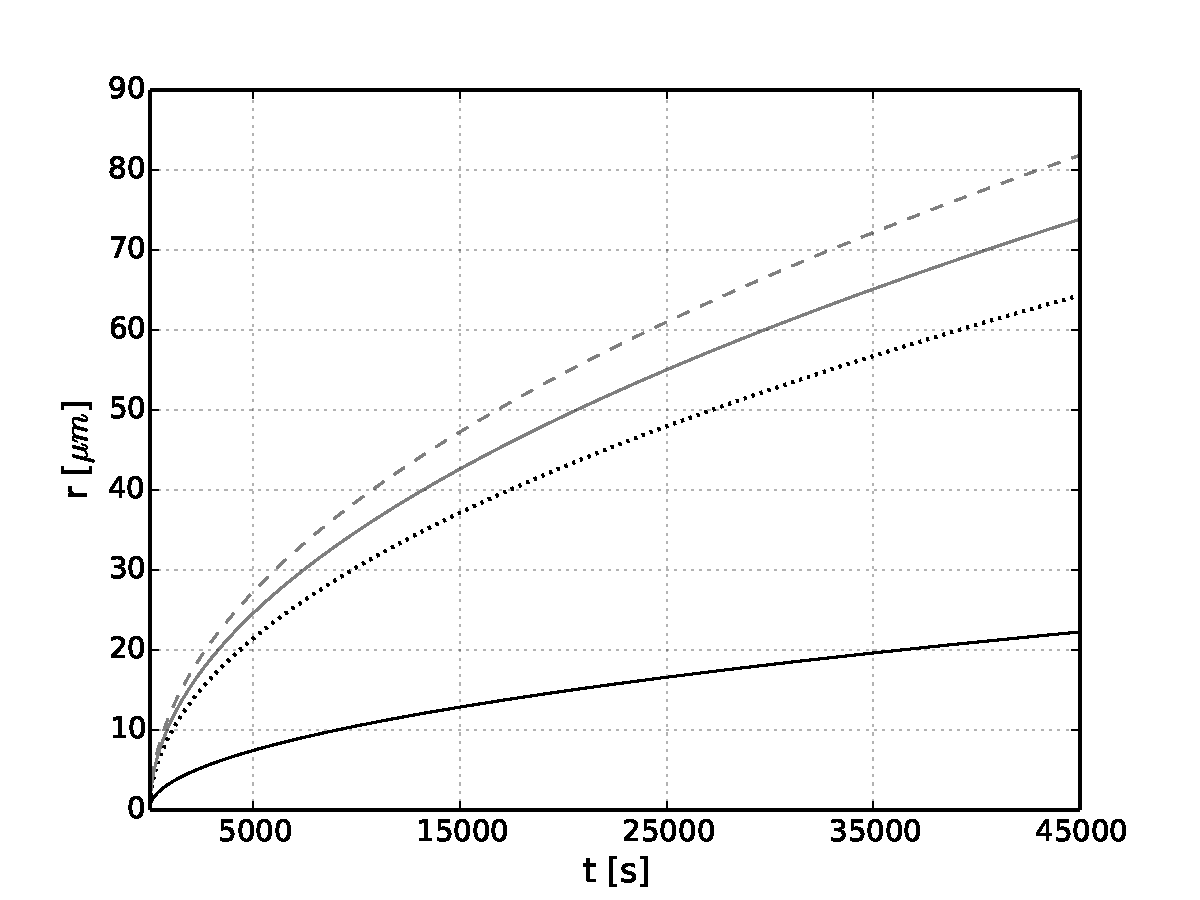
\includegraphics[width=\textwidth]{r_t_temperature.pdf}
    \caption{Droplet growth rate at $p=900 mb$ and $S - 1 = 0.05\%$ as $T$ is increased.}
    \label{fig:temperature}
\end{figure}


\begin{figure}
    \centering
    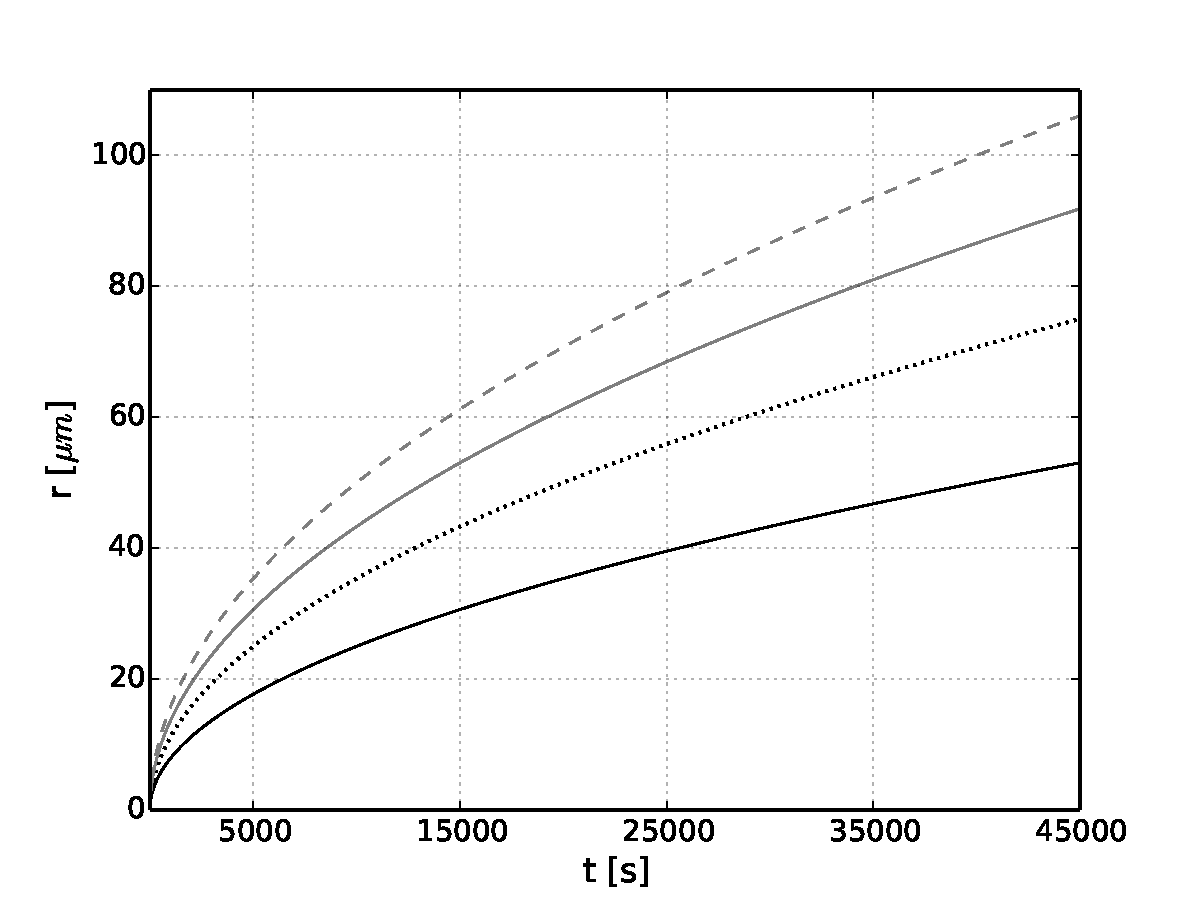
\includegraphics[width=\textwidth]{r_t_supersaturation.pdf}
    \caption{Droplet growth rate at $p=900 mb$ and $T= 273 K$ as the $S - 1$ is increased.}
    \label{fig:supersaturation}
\end{figure}


%--------------------------------------------------
% CONCLUSION
%--------------------------------------------------
\section{Conclusion}
We have evaluated a simplified model of droplet growth rate in warm clouds.
Although the model ignores curvature and solute effects, the model is still
able to capture the general trends of droplet growth, as validated against
droplet growth values from \cite{Curry, Mason, Best} that include curvature and
solute effects. Sensitivity analysis of the model to changes in ambient temperature $T$
and supersaturation $(S -1)$ show a positive relationship between the droplet growth rate
and $T$, and the droplet growth rate and $(S - 1)$.



%--------------------------------------------------
% BIBLIOGRAPHY
%--------------------------------------------------
\bibliography{sources}
\bibliographystyle{plainnat}


\end{document}
